\subsubsection{Layerwise results}
\label{app:vit-common}
The common protocol recovers the same 6,190 exact directions in all three seeds (Table~\ref{tab:vit-common}). Feature-null edits account for the first MLP layer and readout; the second MLP layer contributes downstream-null LayerNorm shifts. No additional selective directions are found.

\begin{table}[!htbp]\centering
\caption{ViT family dimensions under the common protocol (Appendix~\ref{app:methods-common-families}). Slash-separated entries give seeds 0/1/2; selective and approximate dimensions exclude exact-family overlap.}
\label{tab:vit-common}
\small\setlength{\tabcolsep}{5pt}
\begin{tabular}{lrrr}\toprule
Family & First MLP layer & Second MLP layer & Readout\\\midrule
Feature-null & 3,072 & 0 & 45\\
Additional downstream-null & 0 & 3,073 & 0\\
Additional selective & 0 & 0 & 0\\\midrule
Feature tail & 0 & 3,068/1,534/2,301 & 0\\
Downstream tail & 768/768/0 & 0 & 0\\\bottomrule
\end{tabular}
\end{table}

All sampled exact-family edits remain at the numerical floor through radius 1,000. Approximate feature and downstream families also permit larger displacements than matched controls, but show finite crossings (Figure~\ref{fig:vit-common-rays}). The second-layer feature tail crosses by radius 100 in every seed; the first-layer downstream tail crosses by radius 3 where nonempty. The latter is empty in seed 2, with its smallest rate just above the selection cutoff.

\begin{figure}[!htbp]\centering
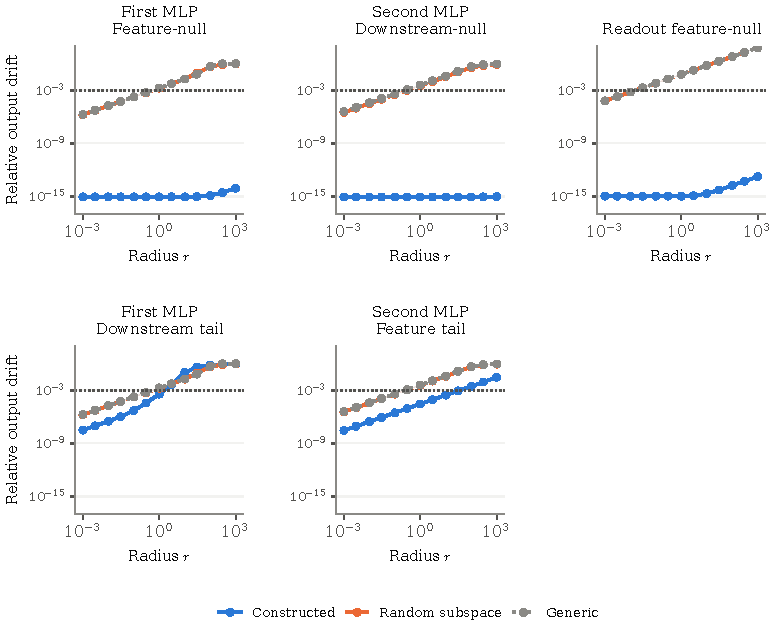
\includegraphics[width=4.670in]{vit_common_rays.pdf}
\caption{ViT common-family ray responses. Curves show the mean of within-seed median relative RMS drift; bands show one sample SD across available seeds. The horizontal line marks $10^{-3}$. Exact-family responses remain at the numerical floor. Controls use the same edited layer and normalization.}
\label{fig:vit-common-rays}\label{tab:vit-common-radii}
\end{figure}
